\documentclass[a4paper,12pt]{article}
\usepackage[russian, english]{babel}

\babelfont{rm}{Times New Roman}
\babelfont{sf}{Times New Roman}

\usepackage[hidelinks]{hyperref}
\usepackage{indentfirst}
\usepackage{listings}
\usepackage{xcolor}
\usepackage{here}
\usepackage{array}
\usepackage{multirow}
\usepackage{graphicx}
% многостраничные таблицы
\usepackage{longtable}
\usepackage[fleqn]{amsmath}
\usepackage{amssymb}
\usepackage{csvsimple}
\usepackage{caption}
\usepackage{pdfpages}
% captionof
% toprule bottomrule etc.
\usepackage{booktabs}
% side-by-side images
\usepackage{caption}
\usepackage{subcaption}
% enumerate biblio
\usepackage[nottoc,numbib]{tocbibind}
% sort alpha
\usepackage[backend=biber,sorting=none,style=ieee,citestyle=ieee]{biblatex}

\renewcommand{\lstlistingname}{Программа} % заголовок листингов кода

\usepackage{listings}

\definecolor{mauve}{rgb}{0.58,0,0.82}

\lstset{frame=shadowbox,
  rulesepcolor=\color{gray},
  language=Python,
  aboveskip=3mm,
  belowskip=3mm,
  showstringspaces=false,
  columns=flexible,
  basicstyle={\ttfamily},
  numbers=none,
  numberstyle=\color{black},
  keywordstyle=\color{blue},
  commentstyle=\color{green},
  stringstyle=\color{mauve},
  breaklines=true,
  breakatwhitespace=true,
  tabsize=3,
  xleftmargin=2em,
  framexleftmargin=2em,
  numbers=left,
  firstnumber=1,
  captionpos=b,
  extendedchars=\true,
  keepspaces=true,
  inputpath=../decision_theory,                     % директория с листингами
}


\usepackage[left=2cm,right=2cm,
top=2cm,bottom=2cm,bindingoffset=0cm]{geometry}

%% Нумерация картинок по секциям
\usepackage{chngcntr}
\counterwithin{figure}{section}
\counterwithin{table}{section}

%%Точки нумерации заголовков
\usepackage{titlesec}
\titlelabel{\thetitle.\quad}
\usepackage[dotinlabels]{titletoc}

%% Оформления подписи рисунка
\addto\captionsrussian{\renewcommand{\figurename}{Рисунок}}
\captionsetup[figure]{labelsep = period, justification=centering}

%% Подпись таблицы
\addto\captionsrussian{\renewcommand{\tablename}{Таблица}}
\captionsetup[table]{labelsep = period, justification=centering}

%% Подпись таблицы
%\DeclareCaptionFormat{hfillstart}{\hfill#1#2#3\par}
%\captionsetup[table]{format=hfillstart,labelsep=newline,justification=centering,skip=-10pt,textfont=bf}

%% Путь к каталогу с рисунками
\graphicspath{{fig/}}

%% Внесение titlepage в учёт счётчика страниц
\makeatletter
\renewenvironment{titlepage} {
 \thispagestyle{empty}
}
\makeatother


\addbibresource{refs.bib}

% magic
\makeatletter
\newcommand{\stackover}{\genfrac{.}{.}\z@{}}
\makeatother

\begin{document}	% начало документа
\selectlanguage{russian}

% Титульная страница
\begin{titlepage}	% начало титульной страницы

	\begin{center}		% выравнивание по центру

		\large Санкт-Петербургский политехнический университет Петра Великого\\
		\large Институт компьютерных наук и технологий \\
		\large Высшая школа программной инженерии\\[8cm]
		% название института, затем отступ 6см
		
		\huge Отчёт по практической работе\\[0.5cm] % название работы, затем отступ 0,5см
		\large ``Модифицированный метод сопряженных градиентов с тремя
		термами и его приложения в задаче восстановления изображений''\\[0.5cm]
		\large по дисциплине "Теория принятия решений"\\[3cm]

	\end{center}

	\begin{flushright} % выравнивание по правому краю
		\begin{minipage}{0.25\textwidth} % врезка в половину ширины текста
			\begin{flushleft} % выровнять её содержимое по левому краю

				\large\textbf{Работу выполнил:}\\
				\large Поздняков А.А.\\
				\large {Группа:} 5130904/00104\\
				
				\large \textbf{Преподаватель:}\\
				\large Черноруцкий И.Г.

			\end{flushleft}
		\end{minipage}
	\end{flushright}
	
	\vfill % заполнить всё доступное ниже пространство
	% \vspace{10\baselineskip}

	\begin{center}
	\large Санкт-Петербург\\
	\large \the\year % вывести дату
	\end{center} % закончить выравнивание по центру

\end{titlepage} % конец титульной страницы



\tableofcontents
\newpage

\section*{Реферат}

При восстановлении изображений часто ставится цель вернуть высококачественную
версию изображения из его более низкокачественной копии. В данной статье мы
рассмотрим один вид задачи восстановления, а именно восстановление фотографий,
искаженных шумами в цифровых изображениях (также известных как шум ''соли и перца'').
При воздействии шума различных частот и интенсивностей (30, 50, 70, 90).
В данной работе мы использовали алгоритм сопряженных градиентов для
восстановления изображений и удаления из них шумов. Мы разработали алгоритм
сопряженных градиентов с тремя ограничениями, используя сопряженное условие Дая
и Ляо, где новый алгоритм достиг условий спуска и глобальной сходимости при
некоторых предположениях. Согласно результатам численного анализа, недавно
созданный подход безусловно превосходит как метод Флетчера и Ривза (FR), так и
метод Флетчера и Ривза с тремя слагаемыми (TTFR). Используется мера структурной
схожести (SSIM), которая применяется для измерения качества изображения, и чем
выше ее значение, тем лучше результат. Исходное изображение сравнивалось со
всеми зашумленными изображениями, а также каждым изображением в соответствии с
процентом шума, а также изображениями, обработанными четырьмя методами.

\section{Введение}

Методы сопряженных градиентов представляют собой мощное семейство алгоритмов
безусловной оптимизации, обладающих отличными локальными и глобальными
свойствами сходимости, используя при этом небольшое количество памяти. Они также
являются быстрыми и эффективными. Исследователи продолжают проявлять сильный
интерес к свойствам сходимости и простоте представления алгоритмов в
компьютерных программах за последние 50 лет и до настоящего дня. Недавно многие
ученые изучают градиентные методы, особенно два типа градиентных методов,
которые недавно привлекли наибольшее внимание. В первом методе используются
условия секущей, которые включают вторичную информацию из целевой функции.

\section{Обзор литературы}

Согласно некоторым исследователям, безусловная оптимизация может быть
рассмотрена как задача поиска минимизационного решения для функционала
$ F\left(\chi\right) $.
\begin{equation}\label{eqn:eq1}
    \min_{\chi \in R^{n}} F \left( \chi \right)    
\end{equation}

где $ F\left( \chi \right) $ - это функция, которая может быть дифференцируемой
хотя бы один раз см. \cite{art1,art2,art3}. Задачу (\ref{eqn:eq1}) можно решить
с помощью алгоритмов сопряженных градиентов (CG), основанных на итерационной
связи, выраженной в:
\begin{equation}\label{eqn:eq2}
    \chi_{k+1}=\chi_{k}+\alpha_{k}\,d_{k}\,k=0,1,2\ldots
\end{equation}

где $ \alpha_{k} $, размер шага в точном или неточном линейном поиске,
вычисляется, когда уравнение является нелинейным, используя следующее
соотношение:
\begin{equation}\label{eqn:eq3}
    F(\chi_{k}+\alpha_{k}\;d_{k})=\min_{a\geq 0}F(\chi_{k}+\alpha_{k}\;d_{k})
\end{equation}

$ d_{k} $ является направлением поиска и определено как:
\begin{equation*}
    d_{1} = -\nabla F_{1}\,k=1
\end{equation*}
\begin{equation}\label{eqn:eq4}
    d_{k+1} = -\nabla F_{k+1}+\beta_{k}\,d_{k}\,k\geq1
\end{equation}

$\nabla F_{k+1}$ - это градиент функции. Основным параметром, используемым в
градиентных методах, является параметр $\beta_{k}$. Далее приведены значения
данного параметра, используемые в соответвующих алгоритмах, данные методы всегда
удовлетворяют условию умеренного спуска, где мы вычисляем $\beta_{k}$ с
направлением поиска $d_{k+1}$. Вот несколько алгоритмов сопряженных градиентов,
включающих следующие параметры: $d_{1} = - \nabla F_{1}, \ y_{k} = \nabla
F_{k+1} - \nabla F_{k}$.
\begin{equation*}
    \beta_{k}^{F R}=\frac{{\cal \nabla}F_{k+1}^{T}{\cal \nabla}F_{k+1}}{{\cal \nabla}F_{k}^{T}{\cal \nabla}F_{k}} \text{\cite{art4}}; \
    \beta_{k}^{P R P}=\frac{y_{k}^{T}\nabla F_{k+1}}{g_{k}^{T}g_{k}}\nonumber \text{\cite{art5}}; \
    \beta_{k}^{H S}=\frac{y_{k}^{T}\nabla F_{k+1}}{\nabla F_{k}^{T}d_{k}} \text{\cite{art6}}; \
\end{equation*}
\begin{equation*}
    \beta_{k}^{\mathrm{DL}}=\frac{y_{k}^{T}\nabla F_{k+1-}\nabla F_{k+1}^{T}s_{k}}{\nabla F_{k}^{T}d_{k}} \text{\cite{art7}},
\end{equation*}

см. \cite{art8,art9,art10,art11,art12,art13,art14,art15}. Существуют варианты
метода, использующие триномиальные сопряженные градиентны, предложенные Чжангом
\cite{art16}. Также значения для параметров алгоритма сопряженных градиентов
(FR) были предложены Полаком-Рибьером (PR) и Хестенсом-Штифелем (HS), данные
алгоритмы также используют триномиальные сопряженные градиенты. Все три
перечисленных метода выполняют условие спуска. Далее приведены значения трёх
слагаемых, используемых в каждом из методов и выражающих их общую схему работы:

\begin{enumerate}
    \item FR
    \begin{equation*}
        d_{k+1}=-\nabla F_{k+1}+\beta^{F R}d_{k}-\theta_{k}^{(1)}\nabla F_{k+1}
    \end{equation*}
    где $ \theta_{k}^{(1)}=\frac{d_{k}^{T}\nabla F_{k+1}}{\nabla F_{k}^{T}\nabla F_{k}} $
    \item PR
    \begin{equation*}
        d_{k+1}=-\nabla F_{k+1}+\beta^{P R P}d_{k}-\theta_{k}^{(1)}\nabla F_{k+1}
    \end{equation*}
    где $\theta_{k}^{(1)}=\frac{d_{k}^{T}\nabla F_{k+1}}{\nabla F_{k}^{T}\nabla F_{k}}$
    \item HS
    \begin{equation*}
        d_{k+1}=-\nabla F_{k+1}+\beta^{H S}d_{k}-\theta_{k}^{(1)}\nabla F_{k+1}
    \end{equation*}
    где $ \theta_{k}^{(1)}=\frac{d_{k}^{T}\nabla F_{k+1}}{d_{k}^{T}y_{k}} $
\end{enumerate}

Заметим, что данные методы удовлетворяют выражению $d_{k}^{T}\mathcal{\nabla
F}_{k}=-||\mathcal{\nabla F}_{k}||^{2}<0,\forall k,$ что означает, что $c = 1$
является достаточным условием для спуска. При изучении сходимости и приложений
метода сопряженных градиентов исследователю часто требуется точное и неточное
направление исследования, такие как усиленные условия Вольфе. Усиленные условия
Вольфе предполагают нахождение $\alpha_{k}$ такого, что
\begin{equation}\label{eqn:eq5}
    F(\chi_{k}+\alpha_{k}d_{k})\leq F(\chi) + n1 \alpha_{k} \nabla F_{k}^{T}d_{k}
\end{equation}
\begin{equation}\label{eqn:eq6}
    |d_{k}^{T}\nabla F_{k}(\chi_{k}+\alpha_{k}d_{k})|\leq-n2\,d_{k}^{T}\nabla F_{k}
\end{equation}

где $0 \le n_{1} \le n_{2} \le 1 $ - это постоянная, установленная в
соответствии с работой Вейджуна и Ли \cite{art17}.

\section{Цели и задачи данного исследования}

В данной работе мы разработали новый алгоритм сопряженных градиентов для решения
задач, связанных с зашумленными изображениями. Задачи, которое были выполнены:

\begin{itemize}
    \item Получить минимальную возможную ошибку по сравнению с похожими методами.
    \item Получить значение индекса структурной схожести (SSIM), близкое к 1,
        демонстрирующее эффективность нового разработанного алгоритма.
    \item Осуществить филтрацию зашумленных изображений с более высокой
        точностью по сравнению с остальными методами, используемыми в данной
        статье.
\end{itemize}

\section{Разработка FR алгоритма с тремя слагаемыми}

В этой части статьи мы улучшаем метод Флетчера и Ривза с тремя слагаемыми (TTFR).
Используя сопряженное условия Дая и Ляо, мы находим новое значение для $\theta$:
\begin{equation*}
    d_{k+1}=-\lambda \nabla F_{k+1}+\beta_{k}^{F R}d_{k}-\theta_{k}\nabla F_{k+1}
\end{equation*}

в зависимости от сопряженного условия Дая и Ляо $ y_{k}^{T}d_{k+1}=-t s_{k}^{T}\nabla F_{k+1} $
значение $ \lambda \le 0 $, and $ t = 1 $ мы находим значение $ \theta_{k}^{NEW}$ \cite{art7},
\begin{equation*}
    y_{k}^{T}d_{k+1}=-\lambda y_{k}^{T}\nabla F_{k+1}+\beta_{k}^{F R}y_{k}^{T}d_{k}-\theta_{k}y_{k}^{T}\nabla F_{k+1}=-s_{k}^{T}\nabla F_{k+1}
\end{equation*}
\begin{equation*}
    \theta_{k}y_{k}^{T}\nabla F_{k+1}=-\lambda y_{k}^{T}\nabla F_{k+1}+\beta_{k}^{F R}y_{k}^{T}d_{k}+s_{k}^{T}\nabla F_{k+1}
\end{equation*}
\begin{equation}\label{eqn:eq7}
    \theta_{k}^{N E W}=-\lambda+\beta_{k}^{F R}\frac{y_{k}^{T}d_{k}}{y_{k}^{T}\nabla F_{k+1}}+\frac{s_{k}^{T}\nabla F_{k+1}}{y_{k}^{T}\nabla F_{k+1}}
\end{equation}
\begin{equation}\label{eqn:eq8}
    d_{k+1}=-\nabla F_{k+1}+\beta_{k}^{F R}d_{k}-\theta_{k}^{N E W} \nabla F_{k+1}
\end{equation}

\noindent План:

\noindent В следующем разделе мы подробно опишем этапы нового алгоритма:

\noindent Этап 1: пусть $x_{0}$ - начальная точка, где $\varepsilon \ge 0$, $k = 0$, 
а затем находим $ d_{0} = -\nabla F_{0} $.

\noindent Этап 2: используя условия Вольфе (\ref{eqn:eq5}), (\ref{eqn:eq6}),
находим значение шага $ \alpha_{k} $.

\noindent Этап 3: если $ \|{\cal \nabla}F_{k+1}\|<\varepsilon $, то завершаем, в
противном случае вычисляем $ x_{k+1} $ из (\ref{eqn:eq2}).

\noindent Этап 4: вычисляем направление поиска из (\ref{eqn:eq7}),
(\ref{eqn:eq8}) и $ \beta_{k}^{FR} $.

\noindent Этап 5: устанавливаем $ k = k + 1 $ и переходим к Этапу 2.

\subsection{Свойство спуска нового метода}

В данном разделе мы докажем достаточное свойство спуска нового алгоритма,
используя параметр FR и подставив новое значение для $\theta_{k}^{NEW}$ в
(\ref{eqn:eq7}). Достаточное условие спуска для методов сопряженных градиентов
записывается следующим образом:
\begin{equation}\label{eqn:eq9}
    \nabla F_{k+1}^{T}d_{k+1}\leq-c\|\nabla F_{k+1}\|^{2}\;\mathrm{for}\;k\geq0\;\mathrm{and}\;c>0
\end{equation}

при этом соблюдение отношений для $k$ и $c$ важно для доказательства
эффективности предложенного алгоритма.

\subsubsection{Теорема}

Для доказательства достаточного условия спуска предложенного алгоритма мы берем
направление поиска, найденное в (\ref{eqn:eq8}) с параметром $\beta_{k}^{FR}$, а
также значение $\theta_{k}$, определенное в (\ref{eqn:eq7}), и получаем
(\ref{eqn:eq2}) для всех значений $k \geq 1$ с использованием (\ref{eqn:eq5}) и
(\ref{eqn:eq6}).

\noindent Доказательство: мы используем математическую индукцию для
доказательства свойства спуска

\begin{itemize}
    \item пусть $k = 0$, тогда $d_{0}=-{\cal \nabla}F_{0}\to{\cal \nabla}F_{0}^{T}d_{0}=-\vert\vert{\cal \nabla}F_{0}\vert\vert^{2}<0$
    \item предположим, что отношение $\nabla F_{k}d_{k}<0$ справедливо для всех $k$
    \item умножим обе стороны уравнения (\ref{eqn:eq8}) на $\nabla F_{k+1}$, тогда уравнение
    (\ref{eqn:eq9}) верно для $k = k + 1$. Имеем:
    \begin{equation*}
        \nabla F_{k+1}^{T}d_{k+1}=-\nabla F_{k+1}^{T}\nabla F_{k+1}+\beta_{k}^{FR}\nabla F_{k+1}^{T}d_{k}-\theta_{k}^{N E W}\nabla F_{k+1}^{T}\nabla F_{k+1}
    \end{equation*}
    \begin{equation*}
        \nabla F_{k+1}^{T}d_{k+1}=-\nabla F_{k+1}^{T}g_{k+1}(1+\theta_{k}^{N E W})+\beta_{k}^{F R}\nabla F_{k+1}^{T}d_{k}
    \end{equation*}
    Если $\theta_{k}^{NEW} \ge 0$, тогда
    \begin{equation*}
        \nabla F_{k+1}^{T}d_{k+1}<-\nabla F_{k+1}^{T}\nabla F_{k+1}(1+\theta_{k}^{N E W})+\beta_{k}^{F R}\nabla F_{k+1}^{T}d_{k}
    \end{equation*}
    \begin{equation*}
        {\cal \nabla}F_{k+1}^{T}d_{k+1}<0
    \end{equation*}
    таким образом, новое и улучшенное условие спуска успешно доказано
\end{itemize}

\subsection{Глобальная сходимость предлагаемого метода}

Теперь мы докажем сходимость нового и известного модифицированного алгоритма в
(\ref{eqn:eq7}) и (\ref{eqn:eq8}) с параметром  $\beta_{k}^{FR}$  FR. Для
исследования сходимости вновь предложенного метода нам необходимо начать с
следующих предположений.

\noindent \textbf{ПРЕДПОЛОЖЕНИЯ (1)}

Будут сделаны следующие предположения относительно задач общей области
(соответствующей области).

\begin{itemize}
    \item $Q=\{\chi\in R^{n}\colon F(\chi)\leq F(\chi_{\circ})\}$ Это
    множество ограниченное и замкнутое.
    \item Функция соответствующей области или области значений дифференцируема и
    непрерывна в определенных $N$ областях множества $q$, и ее производные
    являются непрерывными по Липшицу. Кроме того, непрерывное поведение функции
    соответствующей области или области значений можно увидеть в ее производных.
    Это указывает на наличие фиксированного значения, известного как $D > 0$, и
    его определение следующее:
    \begin{equation*}
        \|\nabla F(\chi)-{\cal \nabla}F(\Upsilon)\|\leq D\|\chi-\Upsilon\|\ \forall\chi,\Upsilon\in N
    \end{equation*}
    \item Функция области $F$ является равномерно выпуклой функцией, где $g$ -
    константа, целое число, которое обеспечивает изменчивость, например,
    \begin{equation*}
        \left(\nabla F(\chi)-\nabla F(\Upsilon)\right)^{T}(\chi-\Upsilon)\geq\mu||\chi-\Upsilon||^{2} \text{, for any} \ \chi,\Upsilon\in Q
    \end{equation*}
\end{itemize}

\noindent Используя предположение (1), с другой стороны, мы находим
положительную константу $B$ в следующем виде:
\begin{equation*}
    \|\chi\|\leq B\ ,\forall\chi\in Q
\end{equation*}
\begin{equation}\label{eqn:eq10}
    \underline{{{\gamma}}}\leq\|\nabla F(\chi)\|\leq\overline{{{\gamma}}}\ ,\forall\chi\in Q
\end{equation}

\noindent \textbf{ЛЕММА (1)}

Мы используем предположения (1) и (\ref{eqn:eq10}), которые выполняются при
взятии (\ref{eqn:eq7}) и (\ref{eqn:eq8}) и использовании усиленных условий Вольфе
для определения размера шага $\alpha_{k}$, предполагая, что наши
предположения верны, если
$\textstyle\sum_{k>1}{\frac{1}{||d_{k+1}||^{2}}}=\infty$, имеем
\begin{equation*}
    \text{имеем} \lim_{k \rightarrow \infty}\left(i n f\lVert\nabla F_{k}\rVert\right)=0
\end{equation*}

\subsubsection{Теорема}

Свойство спуска подтверждает предположение из (1) и (\ref{eqn:eq10}). Метод сопряженных
градиентов, вместе с параметром $\beta_{K}^{FR}$ и $\theta_{k}$, предоставляется
уравнением (\ref{eqn:eq7}), как если бы $\alpha_{k}$ удовлетворяло усиленным условиям Вольфе
(WSC) (\ref{eqn:eq5}) и (\ref{eqn:eq6}) соответственно. Она равномерно выпукла в области $Q$,
следовательно, функция, уравнение 
$\lim_{k \rightarrow \infty} inf||g_{k}|| = 0$, удовлетворяет.

\noindent \textbf{Доказательство:}
\begin{equation*}
    \lVert d_{k+1} \rVert = \lVert -\nabla F_{k+1}+\beta_{k}^{F R}d_{k}-\theta_{k}^{N E W} \nabla F_{k+1} \rVert
\end{equation*}
\begin{equation*}
    \|d_{k+1}\|\leq\|\nabla F_{k+1}\|+\beta_{k}^{F R}\|d_{k}\|+\theta_{k}^{N E W}\|\nabla F_{k+1}\|
\end{equation*}
\begin{equation*}
    ||d_{k+1}||\leq||\nabla F_{k+1}||(1+\theta_{k}^{N E W})+\frac{||\nabla F_{k+1}|^{2}}{||\nabla F_{k}||^{2}}||d_{k}||
\end{equation*}
\begin{equation*}
    ||d_{k+1}||\leq\left(\left(1+\theta_{k}^{N E W}\right)+\frac{||\nabla F_{k+1}||}{||\nabla F_{k}||^{2}}\,||d_{k}||\right)||\nabla F_{k+1}||
\end{equation*}
\begin{equation*}
    \sum_{k \geq 1}{\frac{1}{\left|\left|d_{k+1}\right|\right|}} \geq \left( 
        \frac{1}{
            \left(
                \left(1 + \theta_{k}^{N E W}\right) + 
                \frac{\lVert \nabla F_{k+1} \rVert}{\lVert \nabla F_{k} \rVert^{2}}\lVert d_{k} \rVert
            \right)^{2}
        }
    \right) \frac{1}{\gamma^{2}}\Sigma\mathbf{1} = \infty
\end{equation*}

\noindent используя лемму, представленную ранее, 
$\lim_{k \rightarrow \infty} \lVert \nabla F_{k} \rVert$

\section{Результаты экспериментов и обсуждения}

Изображение обычно искажается из-за шума, возникающего либо в процессе съемки,
либо при передаче изображения. Эффективные решения для снижения шума необходимы
для достижения более надежных результатов в широком спектре приложений,
связанных с изображениями. В данной части статьи мы рассмотрим метод
восстановления исходного изображения изнутри изображения, которое было
повреждено ложным импульсным шумом. Речь идет об изображении, которое пострадало
от ложного импульсного шума. Импульсный шум, который возникает, когда
воздействию подвергается только малая часть пикселя, является одним из наиболее
распространенных типов шума и одним из самых явных. Из-за шума любая информация
о фактических значениях затронутых пикселей полностью уничтожается. Эти
трудности считаются одними из самых сложных с точки зрения областей улучшения
из-за своих гладких характеристик. Это связано с тем, что сложно найти решение
для данных проблем. Особенно трудно найти решения для несглаженных задач
оптимизации из-за того, что многие существующие методы градиента не могут быть
применены напрямую. Поэтому необходимо создавать оригинальные алгоритмы или
подходы для решения этих трудностей. В этой связи Юань и др.
\cite{art18,art19,art20,art21} описывают ряд нелинейных алгоритмов сопряженных
градиентов, которые могут использоваться для несглаженных задач оптимизации.
Большое количество хороших результатов было получено с использованием данных
методов, дополнительные результаты могут быть найдены в задачах
\cite{art22,art23,art24,art25,art26}, и ... Пусть:
\begin{equation*}
    Y=\{(k,m)\in\Lambda\mid\bar{\xi}_{k,m}\neq\xi_{k,m},\xi_{k,m}=\delta_{m i n} \text{or} \delta_{m a x}\}
\end{equation*}

будет индексным множеством шумовых кандидатов, а $x$ - настоящим изображением с
$\left( X, Y \right)$ пикселями, $x_{k,m}$ - оттенком серого цвета $x$ в
указанной позиции пикселя $\left( k, m \right)$ с
$(k,m)\in\Lambda=\{1,2,\cdots,X\}\times\{1,2,3,\cdots,Y\}$, и $\phi_{k,m}
= \{(k,m\:-\:1),(k,m+1),(k\:-\:1,m),(k\:+\:1,m)\}$ будут в окрестности $\left(k,
m \right)$, где $\xi$ - это наблюдаемое зашумленное изображение $x$, искаженное
шумом ''соли и перца'', $\overline{{\xi}}$ определено как изображение, созданное
применением адаптивного медианного фильтра (MED) к зашумленному изображению $y$,
где $\delta_{\min}$ указывает минимальное значение шумового пикселя, а $\delta_{\max}$ -
максимальное значение шумового пикселя. В этом разделе детально рассматриваются
следующие вопросы восстановления изображения, определенные как 
$\min\limits{\nu}\tau \left( \nu \right)$:

\noindent Где:
\begin{equation*}
    \tau(v)=\sum_{(k,m)\in Y}\left\{\Sigma_{(x,y)\in\phi_{k,m}\backslash{N}}\;\chi\bigl(v_{i,j}-\xi_{x,y}\bigr)+\frac{1}{2}\sum_{(x,y)\in\phi_{k,m}\stackover{\cap}{Y}}\;\chi\bigl(v_{k,m}-v_{x,y}\bigr)\right\}
\end{equation*}

\noindent не трудно понять, что регулярность $\tau$ зависит только от $\chi$ и
что функция Хьюбера определена как потенциальная функция для сохранения границы
$\chi$ с тем же значением:
\begin{equation*}
    \chi = \begin{cases} 
        e^{2}/u, \quad \text{если} |e|\leq u \\ 
        |e|-2u, \quad \text{если} |e| \ge u
    \end{cases}
\end{equation*}

\noindent где $u > 0$. Много полезных результатов относительно $\tau$ можно
найти (см. \cite{art24,art25,art26}). Результаты, приведенные ниже, были
получены на персональном компьютере с использованием MATLAB R2021b, процессором
Intel Core i5 с тактовой частотой 2,4 ГГц, 8,00 гигабайтами оперативной памяти и
операционной системой Windows 10. Параметры выбраны как $a = 0,5$, $b = 0,1$, $c
= 0,9$ и $d = 0,3$. Условие остановки:
${\frac{|\tau(v_{k+1})-\tau(v_{k})|}{|\tau(v_{k})|}}<10^{-4}$. Предложенный
фильтр (HM) создан для обработки шума ''соли и перца'' в цифровых изображениях. При
воздействии на изображение шумом с различными коэффициентами
$\left(30,50,70,90\right)$. Зашумленные изображения были подвергнуты фильтрам
(FR, TIFR, а затем медианный фильтр из системы MATLAB) и обработаны для удаления
этого шума. Для демонстрации результатов было выбрано изображение (Lena.png),
известное в литературе и исследованиях по обработке цифровых изображений. К нему
был добавлен шум с различными коэффициентами $\left(30,50,70,90\right)$.
Изображение было обработано с использованием четырех коэффициентов шума и
упомянутых фильтров, а также предложенного фильтра. Результаты представлены в
таблице 1. Для измерения качества изображения использовался индекс SSIM, большее
значение индекса означает лучший результат. Сравнение было произведено при
различных значениях процента шума, оригинальное изображение сравнивалось со
всеми зашумленными изображениями, а также с изображениями, обработанными
четырьмя фильтрами. Из таблицы видно, что при коэффициенте шума $30$
изображение, полученное в результате обработки предложенным фильтром, совпало с
оригинальным изображением с отношением ($0.9600$). В то время как обработка фильтрами FR,
TIFR и медианным фильтром дала значения соответственно ($0.8853$), ($0.9168$) и
($0.6993$). То же самое относится к другим коэффициентам шума. При воздействии на
изображение с коэффициентом шума $50$ результат обработки и сравнения с
оригинальным изображением составил ($0.9392$), при воздействии на изображение с
коэффициентом шума $70$ результат сравнения с оригинальным изображением составил
($0.8946$), при воздействии на изображение с коэффициентом шума $90$ результат
составил ($0.7877$).

\begin{table}[H]
    \centering
    \begin{tabular}{ccccccc}
        \hline
        \multicolumn{7}{c}{Lena} \\
        \hline
        Noise & original Image & noise Image & HM & FR & TTFR & median filtering \\
        30 & 1.0000 & 0.0526 & 0.9600 & 0.8853 & 0.9168 & 0.6993 \\
        50 & 1.0000 & 0.0262 & 0.9392 & 0.5419 & 0.8326 & 0.2321 \\
        70 & 1.0000 & 0.0138 & 0.8946 & 0.0885 & 0.7397 & 0.0527 \\
        90 & 1.0000 & 0.0061 & 0.7877 & 0.4311 & 0.6159 & 0.0115 \\
        \multicolumn{7}{c}{Barbara} \\
        Noise & original Image & noise Image & HM & FR & TTFR & median filtering \\
        30 & 1.0000 & 0.0959 & 0.9251 & 0.8305 & 0.9118 & 0.6213 \\
        50 & 1.0000 & 0.0465 & 0.8793 & 0.7180 & 0.7950 & 0.2351 \\
        70 & 1.0000 & 0.0224 & 0.7997 & 0.5255 & 0.6880 & 0.0587 \\
        90 & 1.0000 & 0.0081 & 0.6565 & 0.4141 & 0.5678 & 0.0129 \\
        \hline
    \end{tabular}
    \caption{}
\end{table}

На рисунке 1 изображены результаты работы программы, первый столбец содержит
оригинальное изображение. Второй столбец содержит изображение после воздействия
шума. Третий столбец содержит изображения после их обработки предложенным
фильтром, четвертый столбец содержит изображения, обработанные фильтром (FR),
пятый столбец содержит изображения, обработанные фильтром (TTFR), шестой столбец
показывает обработку медианным фильтром (MED) MATLAB. Третий столбец показывает
качество изображения после его обработки предложенным фильтром и его
соответствие оригинальному изображению. Для подтверждения результатов и точности
предложенного фильтра было введено другое изображение, результаты для которого
представлены на рисунке 2.

\begin{figure}[H]
    \centering
    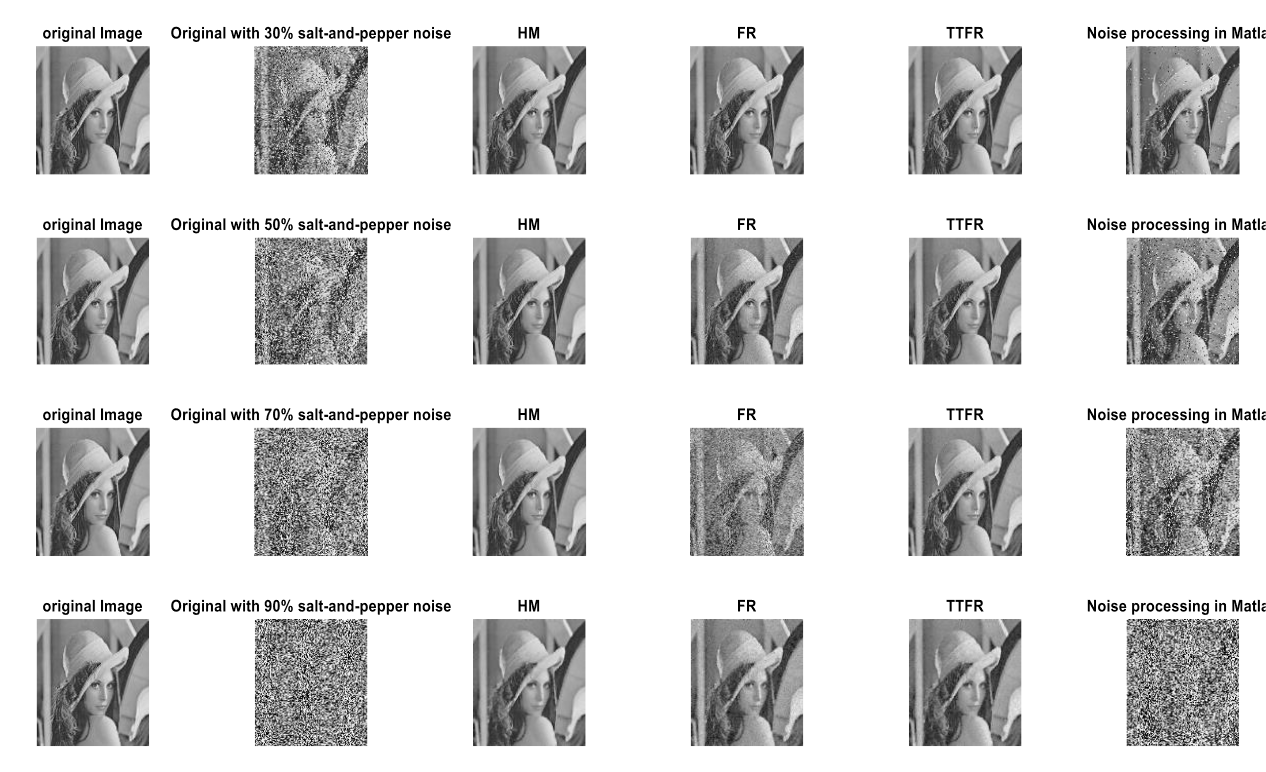
\includegraphics[width=\linewidth]{lena.png}
    \caption{Сравнение результатов удаления шума (Lena.png) 
    с использованием предложенного фильтра и других фильтров}
\end{figure}

\begin{figure}[H]
    \centering
    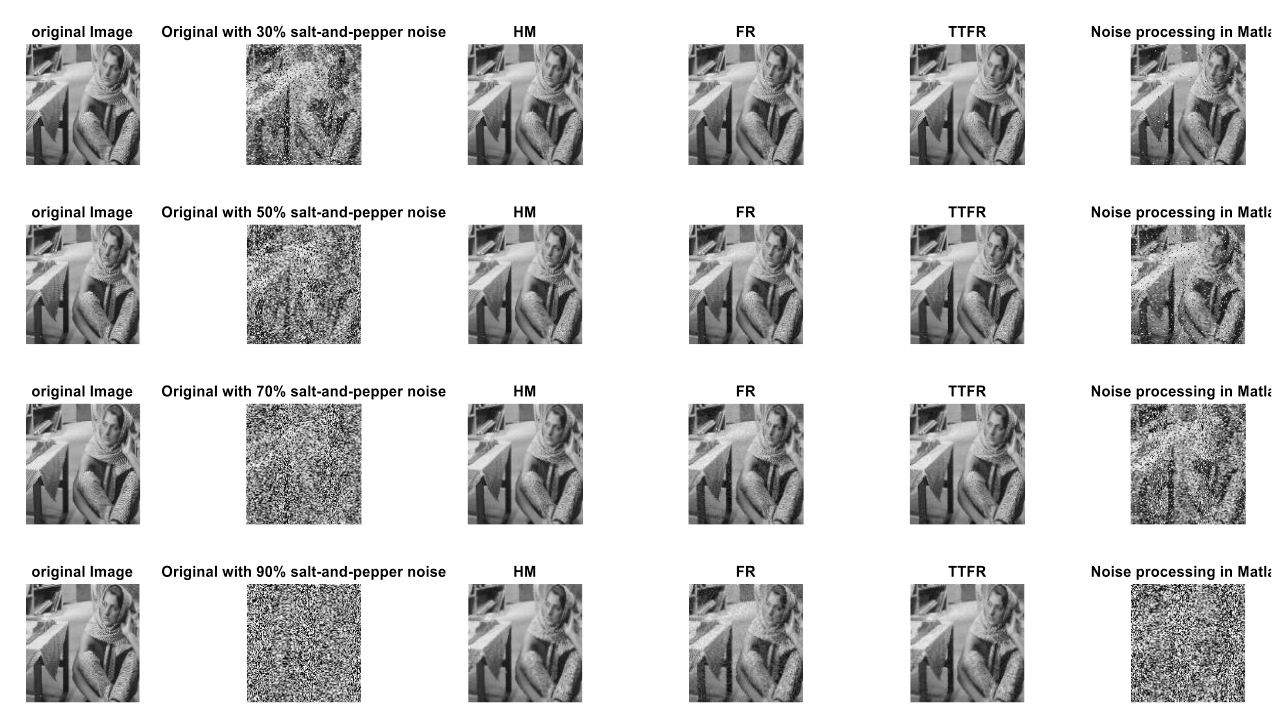
\includegraphics[width=\linewidth]{barbara.png}
    \caption{Сравнение результатов удаления шума (Barbara.png) 
    с использованием предложенного фильтра и других фильтров}
\end{figure}

\section{Вывод}

В данной статье мы обсудили различные методы фильтрации для уменьшения шума ''соли и перца'' на изображениях в оттенках серого. Кроме того, мы представили и сравнили
результаты различных методов фильтрации шума, таких как медианные фильтры и
фильтры, основанных на методах (FR) и (TTFR). Фильтр, основанный на предложенном
методе (HM), обеспечивает лучшую производительность по сравнению с другими
рассмотренными фильтрами (без шумов) и качество изображения в целом. Основные
преимущества этого фильтра заключаются в успешной способности удаления
поврежденных серых пикселей. Однако, данный метод увеличивает вычислительную
сложность. Будущие исследования будут сосредоточены на других фильтрах,
основанных на математических методах, для борьбы с другими типами шумов, а также
на расширении алгоритма для цветных изображений. В данной работе была получена
крайне низкая ошибка по сравнению с другими алгоритмами в этой статье. Значение
SSIM было близко к единице, как подробно указано в числовых результатах. Метод
показал лучшие результаты фильтрации зашумленных изображений по
сравнению с алгоритмами FR и TTFR.

\section{Благодарность}

Выражаю благодарность и признание колледжу компьютерных наук и математики, а
также колледжу фундаментальных наук университета Мосула.

\newpage
\printbibliography[heading=bibintoc]

\end{document}
